\documentclass{beamer}
\usepackage{csc}
\title[ООП]{Лекция 8. Объектно-ориентированное программирование}

\date{
   \textbf{CS центр}\\
   17 октября 2017 \\
   Санкт-Петербург
}

\begin{document}
\begin{frame} 
  \titlepage
\end{frame}

\begin{frame}[fragile]{Ещё раз об ООП}

    {\em Объектно-ориентированное программирование} — 
    концпеция программирования, основанная на
    понятиях объектов и классов.

   \begin{block}{Основные принципы:}
   \begin{itemize}
       \item инкапсуляция,
       \item наследование,
       \item полиморфизм,
       \item абстракция.
   \end{itemize}
   \end{block}

   Подробнее о принципах проектирования ООП-программ
   можно узнать по ключевым слову ,,шаблоны проектирования''.
\end{frame}

\begin{frame}[fragile]{Как правильно построить иерархию?}

    Иерархия геометрических фигур:

\begin{center}
    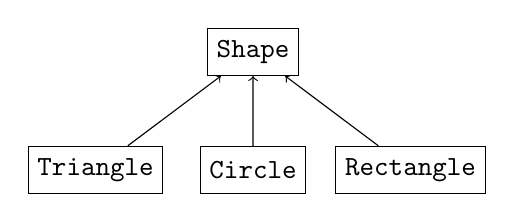
\begin{tikzpicture}[level 1/.style={sibling distance=20mm},minimum height=6mm]
\node (g1) [draw,->] {\tt Shape}
    child[<-]{node [draw] (s1) {\tt Triangle}}
    child[<-]{node [draw] (s2) {\tt Circle}}
    child[<-]{node [draw] (s3) {\tt Rectangle}};
\end{tikzpicture}
\end{center}
\vspace{2cm}

Куда добавить класс {\tt Square}?
\end{frame}

\begin{frame}[fragile]{Как правильно построить иерархию?}
    Квадрат — это прямоугольник, у которого все стороны равны.
\begin{center}
    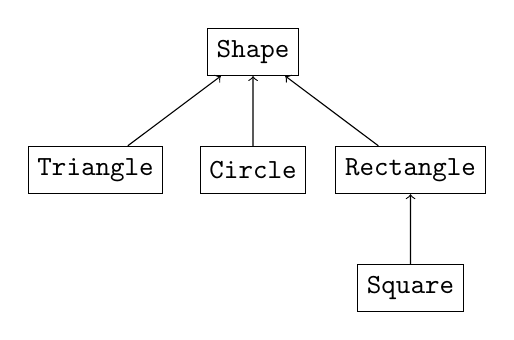
\begin{tikzpicture}[level 1/.style={sibling distance=20mm},minimum height=6mm]
\node (g1) [draw,->] {\tt Shape}
    child[<-]{node [draw] (s1) {\tt Triangle}}
    child[<-]{node [draw] (s2) {\tt Circle}}
    child[<-]{node [draw] (s3) {\tt Rectangle}
        child[<-]{node [draw] (s4) {\tt Square}}};
\end{tikzpicture}
\end{center}
\vspace{-2mm}
\begin{lstlisting}
void double_width(Rectangle & r) {
    r.set_width(r.width() * 2);
}
\end{lstlisting}
\end{frame}

\begin{frame}[fragile]{Как правильно построить иерархию?}
    Прямоугольник задаётся двумя сторонами, а квадрат — одной.
\begin{center}
    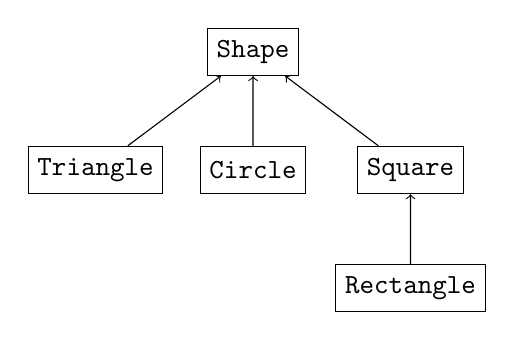
\begin{tikzpicture}[level 1/.style={sibling distance=20mm},minimum height=6mm]
\node (g1) [draw,->] {\tt Shape}
    child[<-]{node [draw] (s1) {\tt Triangle}}
    child[<-]{node [draw] (s2) {\tt Circle}}
    child[<-]{node [draw] (s3) {\tt Square}
        child[<-]{node [draw] (s4) {\tt Rectangle}}};
\end{tikzpicture}
\end{center}

\begin{lstlisting}
double area(Square const& s) {
    return s.width() * s.width();
}
\end{lstlisting}
\end{frame}

\begin{frame}[fragile]{Как правильно построить иерархию?}
    Правильное решение — сделать эти классы независимыми:
\begin{center}
    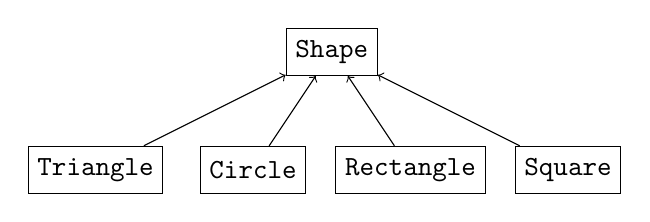
\begin{tikzpicture}[level 1/.style={sibling distance=20mm},minimum height=6mm]
\node (g1) [draw,->] {\tt Shape}
    child[<-]{node [draw] (s1) {\tt Triangle}}
    child[<-]{node [draw] (s2) {\tt Circle}}
    child[<-]{node [draw] (s3) {\tt Rectangle}}
    child[<-]{node [draw] (s4) {\tt Square}};
\end{tikzpicture}
\end{center}
\end{frame}

\begin{frame}[fragile]{Агрегирование vs наследование}
    \begin{itemize}
        \item {\em Агрегирование} — это включение объекта одного 
            класса в качестве поля в другой.

        \item Наследование устанавливает более сильные связи
            между классами, нежели агрегирование:
            \begin{itemize}
                \item приведение между объектами,
                \item доступ к {\tt protected} членам.
            \end{itemize}

        \item Если наследование можно заменить легко на агрегирование,
            то это нужно сделать.
    \end{itemize}
\begin{block}{Примеры некорректного наследования}
\begin{itemize}
    \item Класс {\tt Circle} унаследовать от класса {\tt Point}.
    \item Класс {\tt LinearSystem} унаследовать от класса {\tt Matrix}.
\end{itemize}
\end{block}
\end{frame}

\begin{frame}[fragile]{Принцип подстановки Барбары Лисков}
\begin{block}{Liskov Substitution Principle (LSP)} 
\em\centering  Функции, работающие с базовым классом, должны иметь 
    возможность работать с подклассами не зная об этом.
\end{block}
\vspace{5mm}
    
Этот принцип является важнейшим критерием при построении иерархий наследования. 

\begin{block}{Другие формулировки}
\begin{itemize}
    \item Поведение наследуемых классов не должно противоречить поведению,
            заданному базовым классом.
    \item Подкласс не должен требовать от вызывающего кода больше, чем базовый
        класс, и не должен предоставлять вызывающему коду меньше, чем базовый
        класс 
\end{itemize}
\end{block}
\end{frame}

\begin{frame}[fragile]{Модификаторы при наследовании}
    При наследовании можно использовать модификаторы доступа:
\begin{lstlisting}
    struct A {};
    struct B1 : public A {};
    struct B2 : private A {};
    struct B3 : protected A {};
\end{lstlisting}
Для классов, объявленных как \code{struct}, по-умолчанию используется
\code{public}, для объявленных как \code{class}~— \code{private}.
\vspace{3mm}

{\bf Важно:} {\em отношение наследования} (в терминах ООП) задаётся только \code{public}-наследованием.
\vspace{3mm}

Использование \code{private}- и \code{protected}-наследований целесообразно,
если необходимо не только агрегировать другой класс, но и переопределить его виртуальные методы.
\end{frame}

\begin{frame}[fragile]{Переопределение \code{private} виртуальных методов}
    \begin{lstlisting}[basicstyle=\fontsize{9pt}{1em}\ttfamily,commentstyle=\fontsize{9pt}{1em}\ttfamily\color{MOOCGreen}]
struct NetworkDevice {
    void send(void * data, size_t size) {
        log("start sending");
        send_impl(data, size);
        log("stop sending");
    }
    ...
private:
    virtual void send_impl(void * data, size_t size) 
    {...}
};

struct Router : NetworkDevice {
private:
    void send_impl(void * data, size_t size) {...}
};
    \end{lstlisting}
\end{frame}

\begin{frame}[fragile]{Реализация чистых виртуальных методов}
    Чистые виртуальные методы могут иметь определения:
    \begin{lstlisting}[basicstyle=\fontsize{9pt}{1em}\ttfamily,commentstyle=\fontsize{9pt}{1em}\ttfamily\color{MOOCGreen}]
struct NetworkDevice {
    virtual void send(void * data, size_t size) = 0;
    ...
};

void NetworkDevice::send(void * data, size_t size) {
    ...
}

struct Router : NetworkDevice {
    void send(void * data, size_t size) {
        // невиртуальный вызов
        NetworkDevice::send(data, size);
    }
};
    \end{lstlisting}
\end{frame}

\begin{frame}[fragile]{Интерфейсы}{}
    {\em Интерфейс}~— это абстрактный класс, у которого отсутствуют поля,
    а все методы являются чистыми виртуальными.

    \begin{lstlisting}
struct IConvertibleToString {
    virtual ~IConvertibleToString() {}
    virtual string toString() const = 0;
};
    \end{lstlisting}
    \begin{lstlisting}
struct IClonable {
    virtual ~IClonable() {}
    virtual IClonable * clone() const = 0;
};
    \end{lstlisting}
    \begin{lstlisting}
struct Person : IClonable {
    Person * clone() {return new Person(*this);}
};
    \end{lstlisting}
\end{frame}

\begin{frame}[fragile]{Множественное наследование}

    В \langcpp разрешено множественное наследование.
\begin{lstlisting}
    struct Person {};
    struct Student : Person {};
    struct Worker  : Person {};
    struct WorkingStudent : Student, Worker {};
\end{lstlisting}
    Стоит избегать {\em наследования реализаций} более чем от одного 
    класса, вместо этого использовать интерфейсы.

\begin{lstlisting}
    struct IWorker {};
    struct Worker : Person, IWorker {};
    struct Student : Person {};
    struct WorkingStudent : Student, IWorker {};
\end{lstlisting}

Множественное наследование — это отдельная большая тема.
\end{frame}

\begin{frame}[fragile]{Дружественные классы}
\begin{lstlisting}
struct String {
    ...
    friend struct StringBuffer;
private:
    char * data_;
    size_t len_;
};

struct StringBuffer {
    void append(String const& s) {
        append(s.data_);
    }
    void append(char const* s) {...}
    ...
};                   
\end{lstlisting}
\end{frame}

\begin{frame}[fragile]{Дружественные функции}{}
    Дружественные функции можно определять прямо внутри описания
    класса (они становятся \code{inline}).
\begin{lstlisting}
struct String {
    ...
    
    friend void print(String const& s) 
    {
        os << s.data_;
    }

private:
    char * data_;
    size_t len_;
};                   
\end{lstlisting}
\end{frame}

\begin{frame}[fragile]{Дружественные методы}
\begin{lstlisting}
struct String;
struct StringBuffer {
    void append(String const& s);
    void append(char const* s) {...}
    ...
};                   

struct String {
    ...
    friend 
      void StringBuffer::append(String const& s);
};
        
void StringBuffer::append(String const& s) {
    append(s.data_);
}
\end{lstlisting}
\end{frame}

\begin{frame}[fragile]{Отношение дружбы}
    Отношение дружбы можно охарактеризовать следующими 
    утверждениями: 
    \begin{itemize}
        \item Отношение дружбы не симметрично.
        \item Отношение дружбы не транзитивно.
        \item Отношение наследования не задаёт
            отношение дружбы.
        \item Отношение дружбы сильнее, чем 
            отношение наследования. 
    \end{itemize}
    \begin{block}{Вывод}
        Стоит избегать ключевого слова \code{friend}, так как оно нарушает
        инкапсуляцию.
    \end{block}
\end{frame}

\end{document}

 
